
% This LaTeX was auto-generated from MATLAB code.
% To make changes, update the MATLAB code and republish this document.

\documentclass{article}
\usepackage{graphicx}
\usepackage{color}

\sloppy
\definecolor{lightgray}{gray}{0.5}
\setlength{\parindent}{0pt}

\begin{document}

    
    
\subsection*{Contents}

\begin{itemize}
\setlength{\itemsep}{-1ex}
   \item Zachary Kaplan
   \item Parabolic PDE Instance
   \item C.4.1.1 - Dimensionless PDE
   \item C.4.1.2 - Spatial Discretization
   \item C.4.1.3 - Temporal Discretization
   \item C.4.1.4 - ode23 vs. ode23s
   \item C.4.1.5 - Jacobian Hinting
   \item C.4.1.6 - Visualize \& Review
   \item Concluding Remarks
   \item Helper Functions
\end{itemize}


\subsection*{Zachary Kaplan}

\begin{par}
Math 440 Computational Lab \#3 4/11/19
\end{par} \vspace{1em}
\begin{verbatim}
%
% An online version of this file can be found published to:
% https://www.overleaf.com/read/zgmxqsryykhj
%
% *NOTE*: To render this file locally, please prepend the following package
%         dependencies to the latex generated by matlab publish:
%
%  \usepackage[margin=1in]{geometry}
%  \usepackage{amsmath}
%  \usepackage{amssymb}
%  \usepackage{microtype}
%  \usepackage{csquotes}
%  \usepackage{bm}
%
\end{verbatim}


\subsection*{Parabolic PDE Instance}

\begin{par}
In this lab, we will consider the PDE describing the diffusion of heat through a metallic rod.
\end{par} \vspace{1em}
\begin{par}
Let $L$ [ $m$ ] denote the length of the rod, $T$ [ $C$ ] denote the temperature of the rod across space and time, $\rho$ [ $kg/m^3$ ] denote the density of the rod, $C_p$ [ $J/(kg \cdot C)$ ] denote the heat capacity of the rod, and $k$ [ $J/(m \cdot s \cdot C)$ ] denote the thermal conductivity of the rod. We will consider this physical system over the 1-D spatial domain $x \,[m] \in \Omega = (0, L)$, and the temporal domain $t\,[s] \in (0, \infty)$. The following PDE then describes the difussion of heat through the rod:
\end{par} \vspace{1em}
\begin{par}
$$
  \rho C_p \frac{\partial T}{\partial t} =
      k \frac{\partial^2 T}{\partial x^2},
      \quad \forall (x, t) \in \Omega \times (0, \infty).
$$
\end{par} \vspace{1em}
\begin{par}
We want to consider this rod where a temperature step-pulse of amplitude $T_0$ occurs at the left endpoint $x = 0$ for time $t \in (0, t_p)$. On the right endpoint, we consider the rod to be isolated and so heat does not flow through where $x = L$. As such, our boundary and initial conditions are:
\end{par} \vspace{1em}
\begin{par}
$$ \begin{gathered}
  T(0, t) =
    \begin{cases} T_0 & 0 \le t \le t_p \\ 0 & t > t_p \end{cases}, \quad
  \frac{\partial T}{\partial x}(L, t) = 0, \\
  T(x, 0) = \begin{cases} T_0 & x = 0 \\ 0 & 0 < x \le L \end{cases}.
\end{gathered} $$
\end{par} \vspace{1em}


\subsection*{C.4.1.1 - Dimensionless PDE}

\begin{par}
In this section, we show that with the proper rescaling of our domain and function $T$, we can represent the above constraints on $T$ with dimensionless equations. Consider dimensionless parameters $\xi$ for space and $\tau$ for time, and the dimensionless function $u$ where
\end{par} \vspace{1em}
\begin{par}
$$ \begin{aligned}x = L\xi, && t = t_p\tau, && T = T_0u\end{aligned}. $$
\end{par} \vspace{1em}
\begin{par}
If we look at the endpoints of our original domain we see that $\xi|_{x = 0} = 0, \xi|_{x = L} = 1,   \tau|_{t = 0} = 0, \tau|_{t \to \infty} \to \infty$. As such, our dimensionless spatial domain becomes $\xi \in \hat\Omega = (0, 1)$, and our dimensionless temporal domain becomes $\tau \in (0, \infty)$. We can then write the partials of $T$ in terms of $u$, $\xi$, and $\tau$ as
\end{par} \vspace{1em}
\begin{par}
$$ \begin{aligned}
  \frac{\partial T}{\partial t} &=
    \frac{\partial T_0u}{\partial \tau}\frac{\partial \tau}{\partial t} =
    \frac{T_0}{t_p} \frac{\partial u}{\partial \tau}, \\
  \frac{\partial T}{\partial x} &=
    \frac{\partial T_0u}{\partial \xi^2} \frac{\partial \xi}{\partial x} =
  \frac{T_0}{L} \frac{\partial u}{\partial \xi}, \\
  \frac{\partial^2 T}{\partial x^2} &=
    \frac{\partial^2 T_0u}{\partial \xi^2}
       \left(\frac{\partial \xi}{\partial x}\right)^2 =
  \frac{T_0}{L^2} \frac{\partial^2 u}{\partial \xi^2}.
\end{aligned} $$
\end{par} \vspace{1em}
\begin{par}
Substituting these values into the original PDE, we find
\end{par} \vspace{1em}
\begin{par}
$$ \begin{gathered}
  \rho C_p \frac{T_0}{t_p} \frac{\partial u}{\partial \tau} =
    k \frac{T_0}{L^2} \frac{\partial^2 u}{\partial \xi^2} \\
  \implies \frac{\partial u}{\partial \tau} =
    a \frac{\partial^2 u}{\partial \xi^2},
  \quad (\xi, \tau) \in \hat\Omega \times (0, \infty),
\end{gathered} $$
\end{par} \vspace{1em}
\begin{par}
where
\end{par} \vspace{1em}
\begin{par}
$$ \begin{gathered}
 a = \frac{k t_p}{\rho C_p L^2} ~\text{has units}~
 \left[ \frac{J/(m \cdot s \cdot C) \cdot s}
        {kg/m^3 \cdot J/(kg \cdot C) \cdot m^2} \right] \equiv
 \left[ \frac{J}{J} \frac{1/m}{1/m^3 \cdot m^2} (1/s \cdot s)
   \frac{1/C}{1/C} \frac{1}{kg \cdot 1/kg} \right] \equiv [1]. \\
 \therefore a~\text{is dimensionless}.
\end{gathered} $$
\end{par} \vspace{1em}
\begin{par}
We can also substitute these equations into the boundary and initial conditions to obtain
\end{par} \vspace{1em}
\begin{par}
$$ \begin{aligned}
  T(0 = x(0), t(\tau)) &=
  \begin{cases}
    T_0 & 0 \le t_p \tau \le t_p \\ 0 & t_p \tau > t_p
  \end{cases} = T_0 u(0, \tau)
  &&\implies u(0, \tau) =
  \begin{cases}
    1 & 0 \le \tau \le 1 \\ 0 & \tau > 1
  \end{cases}, \\
  \frac{\partial T}{\partial x}(L = x(1), t(\tau)) &= 0 =
    \frac{T_0}{L} \frac{\partial u}{\partial \xi}(1, \tau)
  &&\implies \frac{\partial u}{\partial \xi}(1, \tau) = 0, \\
  T(x(\xi), 0 = t(0)) &=
    \begin{cases} T_0 & L\xi = 0 \\ 0 & 0 < L\xi \le L \end{cases} =
  T_0 u(\xi, 0)
  &&\implies u(\xi, 0) =
    \begin{cases} 1 & \xi = 0 \\ 0 & 0 < \xi \le 1
  \end{cases}.
\end{aligned} $$
\end{par} \vspace{1em}
\begin{par}
From this point forward, this lab will only consider this dimensionless problem, fixing the dimensionless parameter $a = 1$.
\end{par} \vspace{1em}


\subsection*{C.4.1.2 - Spatial Discretization}

\begin{par}
We will now discretize the spatial domain of our nondimensional PDE where $\bm{\xi} = \{ \xi_0=0, \xi_1=h, \ldots, \xi_j=jh, \ldots \xi_{N-1}=1,   \xi_N=1+h \}$ are our $N$ grid points with one additional ghost point. If we define $\bm{u}(\tau) = \{u_0(t) \approx u(\xi_0, \tau), u_1(\tau)   \approx u(\xi_1, \tau), \ldots, u_{N-1}(\tau)   \approx u(\xi_{N-1}, \tau), u_N(\tau) \approx u(\xi_N, \tau) \}$, then the following centered finite difference equations hold on the interior of our discrete spatial domain:
\end{par} \vspace{1em}
\begin{par}
$$
  \frac{du_j}{d\tau} = \frac{u_{j-1} - 2u_{j} + u_{j+1}}{h^2} \quad
    \forall j \in \mathbb{Z}_{[1,N-1]}.
$$
\end{par} \vspace{1em}
\begin{par}
Our spatial boundary conditions also follow trivially as either an algebraic equation or as another centered finite diference:
\end{par} \vspace{1em}
\begin{par}
$$ \begin{gathered}
  u_0(\tau) = u(0, \tau) =
    \begin{cases} 1 & 0 \le \tau \le 1 \\ 0 & \tau > 1 \end{cases} \\
  \frac{u_{N} - u_{N-2}}{h} = 0
\end{gathered} $$
\end{par} \vspace{1em}
\begin{par}
Finally, the temportal initial condition translates as
\end{par} \vspace{1em}
\begin{par}
$$ \bm{u}(0) = \{1, 0, 0, \ldots, 0\} $$
\end{par} \vspace{1em}
\begin{par}
since $u(\xi, 0) = 1$ iff $\xi = 0$ and $u(\xi, 0) = 0$ otherwise.
\end{par} \vspace{1em}
\begin{par}
Notice that since $u_0(\tau)$ is given explicitly above, we can substitute $u_0$ out in our overall matrix equation. We can also solve explicitly for $u_N(\tau) = u_{N-2}(\tau)$, allowing for another substitution. With this in mind, we will redefine $\bm{u} = \{u_1(\tau), \ldots, u_{N-1}(\tau)\}$ resulting in
\end{par} \vspace{1em}
\begin{par}
$$
  \frac{d\bm{u}}{d\tau} = A\bm{u} + \bm{b}(\tau), \quad
    \bm{u}(0) = \mathbf{0}
$$
\end{par} \vspace{1em}
\begin{par}
where
\end{par} \vspace{1em}
\begin{par}
$$ \begin{aligned}
  A = \frac{1}{h^2} \begin{pmatrix}
    -2 &  1 &  0 & \cdots &  0 &  0 \\
     1 & -2 &  1 & \cdots &  0 &  0 \\
     0 & \ddots & \ddots & \ddots & & \vdots \\
     \vdots & & \ddots & \ddots & \ddots & 0 \\
     0 & \cdots & 0 & 1 & -2 & 1 \\
     0 & \cdots & 0 & 0 &  2 & -2 \end{pmatrix}
     \in \mathbb{R}^{N-1 \times N-1},
  &&
  \bm{b}(\tau) = \frac{1}{h^2} \begin{pmatrix}
     u_0(\tau) \\ 0 \\ \vdots \\ 0 \end{pmatrix}
     \in \mathbb{R}^{N-1},
  &&
  \bm{u}(0) = \mathbf{0} \in \mathbb{R}^{N-1}.
\end{aligned} $$
\end{par} \vspace{1em}


\subsection*{C.4.1.3 - Temporal Discretization}

\begin{par}
Finally, we discretize $\tau$ using Explicit Euler's Method with a stepsize of $\Delta t$. Let our $\tau$ grid span $[0, \tau_f]$ for some $\tau_f > 0$, and thus we need $M = \tau_f/\Delta t + 1$ grid points. Take $\bm{\tau} = \{\tau_0 = 0, \tau_1 = \Delta t, \ldots   \tau_k = k\Delta t, \ldots, \tau_M = \tau_f\}$ and define $\bm{u}^k \approx \bm{u}(\tau_k)$. We will also define matrix $U$ s.t. $U_{j,k} = u^{k-1}_{j-1}$. Note that our $U$ is the vertical mirror of the text's $U$. We then enforce
\end{par} \vspace{1em}
\begin{par}
$$ \begin{aligned}
 \frac{\bm{u}^{k+1} - \bm{u}^k}{\Delta t} = A\bm{u}^{k} + \bm{b}(\tau_k),
   \quad \forall k \in \mathbb{Z}_{0,M-1},
 &&
 \bm{u}^0 = \bm{0}
\end{aligned} $$
\end{par} \vspace{1em}
\begin{verbatim}
% Picked from later in the lab.
tau_f = 2;

% First, let's try it with N and M on the same order.
N = 10;
M = N;
[xi, tau, U] = mol_ee_solve(N, M, tau_f);
h = xi(2) - xi(1);
dt = tau(2) - tau(1);
figure;
surf(xi, tau, U');
xlabel('\xi', 'Interpreter', 'tex');
ylabel('\tau', 'Interpreter', 'tex');
zlabel('u');
title(sprintf(['Solution where M = O(N)\n' ...
               'h = %f, \\Delta t = %f, \\Delta t / h^2 = %f'], ...
               h, dt, dt/h^2), 'Interpreter', 'tex');

% Now, let's try making M on the order of N^2.
M = 5 * N^2;
[xi, tau, U] = mol_ee_solve(N, M, tau_f);
h = xi(2) - xi(1);
dt = tau(2) - tau(1);
figure;
surf(xi, tau, U', 'LineStyle', ':', 'FaceColor', 'interp');
xlabel('\xi', 'Interpreter', 'tex');
ylabel('\tau', 'Interpreter', 'tex');
zlabel('u');
title(sprintf(['Solution where M = O(N^2)\n' ...
               'h = %f, \\Delta t = %f, \\Delta t / h^2 = %f'], ...
               h, dt, dt/h^2), 'Interpreter', 'tex');

% Save some of this data to plot again later.
plot_later = {xi, tau, U};
\end{verbatim}
\begin{par}
Notice in the surface plots for this section that when $M = O(N)$ we have unstable behavior in the form of spurious oscillations. The solution behaves wildly near $\tau_f$. Instead, when $M = O(N^2)$ we get smooth, sensible behavior. Since the end with $\xi = 1$ is isolated, we see the heat from the initial pulse cause the entire rod to slowly heat up over $\tau \in [0,1]$. Then we see the heat slowly disipate through the endpoint $\xi = 0$ where the heat is fixed at 0.
\end{par} \vspace{1em}

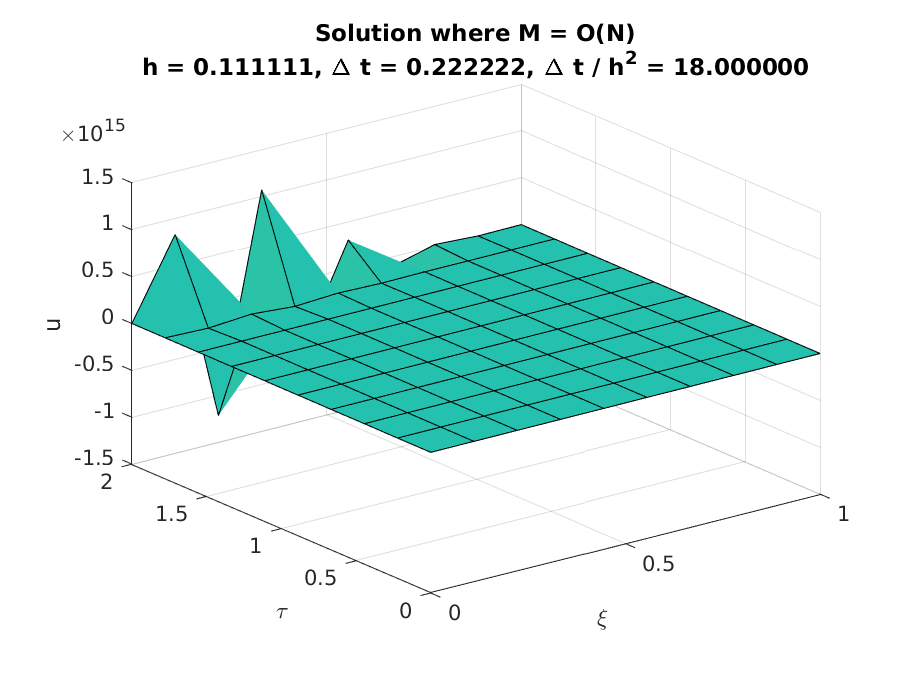
\includegraphics [width=4in]{lab3_01.eps}

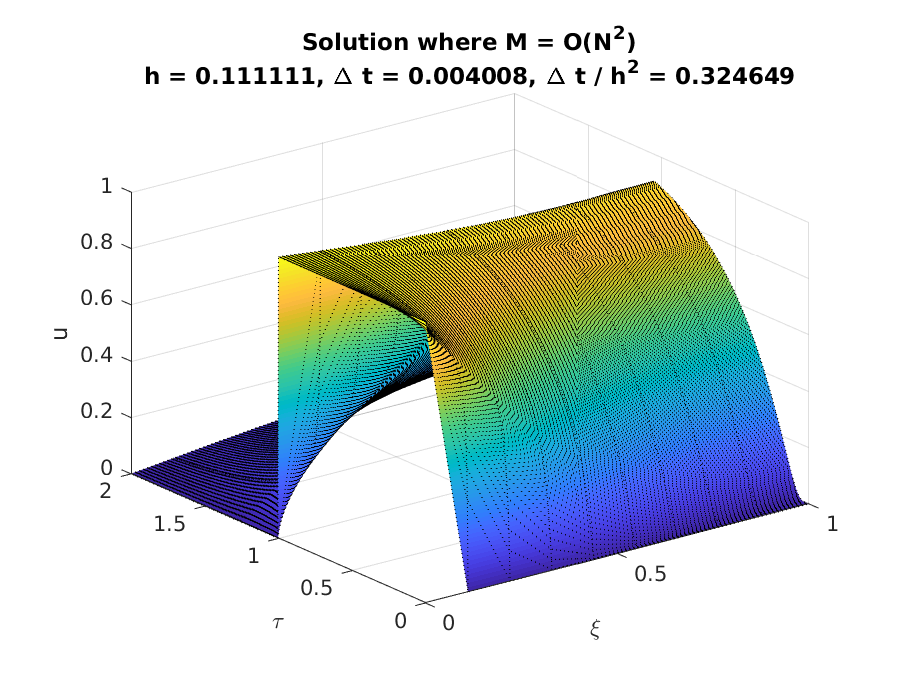
\includegraphics [width=4in]{lab3_02.eps}


\subsection*{C.4.1.4 - ode23 vs. ode23s}

\begin{par}
In this section, we do a case study to help decipher the difference between using ode23 and ode23s.
\end{par} \vspace{1em}
\begin{verbatim}
% Lab specified parameters.
tau_f = 2;
Ns = pow2(10, 0:2);

% Storage for table values.
% Row index is for Ns, column index is for stiffness.
unstiff_idx = 1;
stiff_idx = 2;
table_dim = [numel(Ns), 2];
num_time_steps = zeros(table_dim);
cpu_times = zeros(table_dim);  % in seconds.
max_dt = zeros(table_dim);

for n_idx = 1:numel(Ns)
    % Solve with the unstiff solver.
    t = tic;
    [~, tau, ~] = mol_ode23_solve(Ns(n_idx), tau_f);
    cpu_times(n_idx, unstiff_idx) = toc(t);
    num_time_steps(n_idx, unstiff_idx) = numel(tau);
    max_dt(n_idx, unstiff_idx) = max(diff(tau));

    % Solve with stiff solver.
    t = tic;
    [~, tau, ~] = mol_ode23_solve(Ns(n_idx), tau_f, 'stiff');
    cpu_times(n_idx, stiff_idx) = toc(t);
    num_time_steps(n_idx, stiff_idx) = numel(tau);
    max_dt(n_idx, stiff_idx) = max(diff(tau));
end

% Print the table header.
fprintf('    | %-15s | %-15s | %-15s\n', ...
        'Num Time Steps', 'CPU Time (s)', 'dt_max');
fprintf('  N ');
for i = 1:3
    fprintf('|  ode23 | ode23s ');
end
fprintf('\n');

% Print table rows.
for n_idx = 1:numel(Ns)
    % Table Separator.
    fprintf(['----' repmat(['+' repmat('-', 1, 17)], 1, 3) '\n']);
    % Row Contents.
    fprintf(' %2d | %6d | %6d | %.4f | %.4f | %.4f | %.4f\n', Ns(n_idx),...
        num_time_steps(n_idx, :), cpu_times(n_idx, :), max_dt(n_idx, :));
end

fprintf('\n');
\end{verbatim}
\begin{par}
\textbf{NOTE}: Sorry about the table alignment, seems to be a monospace font issue.
\end{par} \vspace{1em}
\begin{par}
By studying the table, it is clear that the stiff solver is very beneficial for this problem, especially for larger $N$ values. Notice that the number of time steps required seems to grow linearly for \texttt{ode23s} , but quadratically for \texttt{ode23}. Similarly, while CPU time starts out higher for \texttt{ode23s}, it's growth is significantly slower than the growth of \texttt{ode23}, which actually rivals the CPU time of \texttt{ode23s} for $N = 40$. Finally, notice that the maximum $\Delta t$ for \texttt{ode23} seems to drop by a factor of 5 for each doubling of $N$, while \texttt{ode23s}'s maximum $\Delta t$ hardly changes as $N$ doubles.
\end{par} \vspace{1em}

        \color{lightgray} \begin{verbatim}    | Num Time Steps  | CPU Time (s)    | dt_max         
  N |  ode23 | ode23s |  ode23 | ode23s |  ode23 | ode23s 
----+-----------------+-----------------+-----------------
 10 |    285 |    101 | 0.0163 | 0.0353 | 0.0182 | 0.1451
----+-----------------+-----------------+-----------------
 20 |   1170 |    131 | 0.0319 | 0.0447 | 0.0058 | 0.1454
----+-----------------+-----------------+-----------------
 40 |   4862 |    161 | 0.0967 | 0.0851 | 0.0010 | 0.1510

\end{verbatim} \color{black}
    

\subsection*{C.4.1.5 - Jacobian Hinting}

\begin{par}
In this section, we will give hints about the jacobian of the linear system to matlab. Notice that the linear ODE system is
\end{par} \vspace{1em}
\begin{par}
$$
  \frac{d\bm{u}}{d\tau} = f(\tau, \bm{u}) = A\bm{u} + \bm{b}(\tau)
$$
\end{par} \vspace{1em}
\begin{par}
and therefore the jacobian of the system is trivially
\end{par} \vspace{1em}
\begin{par}
$$
  Jf = A.
$$
\end{par} \vspace{1em}
\begin{par}
Since $A$ is tridiagonal, the sparsity pattern of $Jf$ is
\end{par} \vspace{1em}
\begin{par}
$$ \begin{pmatrix}
  1 & 1 & 0 & \cdots & 0 &  0 \\
  1 & 1 & 1 & \cdots & 0 &  0 \\
  0 & \ddots & \ddots & \ddots & & \vdots \\
  \vdots & & \ddots & \ddots & \ddots & 0 \\
  0 & \cdots & 0 & 1 & 1 & 1 \\
  0 & \cdots & 0 & 0 & 1 & 1
\end{pmatrix}. $$
\end{par} \vspace{1em}
\begin{verbatim}
% Lab specified parameters.
tau_f = 2;
Ns = pow2(10, 0:2);

% Configuration Names.
conf_names = {'No Hint', 'JPattern', 'Jacobian'};
% Options for each configuration.
conf_opts = {{'stiff'}, {'stiff', 'jpat'}, {'stiff', 'jacob'}};

% Storage for table values.
% Row index is for Ns, column index is for type of hint.
table_dim = [numel(Ns), numel(conf_names)];
num_time_steps = zeros(table_dim);
cpu_times = zeros(table_dim);  % in seconds.
max_dt = zeros(table_dim);

for n_idx = 1:numel(Ns)
    for c_idx = 1:numel(conf_names)
        % Solve using the proper options.
        t = tic;
        [~, tau, ~] = mol_ode23_solve(Ns(n_idx), tau_f, ...
                                      conf_opts{c_idx}{:});
        cpu_times(n_idx, c_idx) = toc(t);
        num_time_steps(n_idx, c_idx) = numel(tau);
        max_dt(n_idx, c_idx) = max(diff(tau));
    end
end

% Print the table header.
fprintf('    | %-30s | %-30s | %-30s\n', ...
        'Num Time Steps', 'CPU Time (s)', 'dt_max');
fprintf('  N ');
for i = 1:3
    fprintf('| %8s | %8s | %8s ', conf_names{:});
end
fprintf('\n');

% Print table rows.
for n_idx = 1:numel(Ns)
    % Table Separator.
    fprintf(['----' repmat(['+' repmat('-', 1, 32)], 1, 3) '\n']);
    % Row Contents.
    fprintf(' %2d ', Ns(n_idx));
    fprintf('| %8d ', num_time_steps(n_idx, :));
    fprintf('| %.6f ', cpu_times(n_idx, :));
    fprintf('| %.6f ', max_dt(n_idx, :));
    fprintf('\n');
end

fprintf('\n');
\end{verbatim}
\begin{par}
We unsurprisingly see that the more detailed information we give the solver, the more efficiently it is able to preform. Ths first interesting note is that all three types of hinting have no significant effect on the number of time steps. Similarly there is almost no effect on the max $\Delta t$. There is, however, a noticable effect on the CPU time taken. With no hinting at all, \texttt{ode23s}'s runtime seems to grow quadratically, while both with JPattern and the full Jacobian \texttt{ode23s}'s runtime seems to grow linearly. This makes sense because instead of computing an $O(N^2)$ numerical jacobian each iteration, with JPattern \texttt{ode23s} has $O(N)$ numerical values to compute and can evaluate the jacobian in $O(1)$ time when it is supplied as a constant. Of course, the jacobian must also be inverted and this is where a time component of $O(N)$ is picked up even in the case where the jacobian is supplied in full. Since the jacobian is clearly tridiagonal in both the JPattern and full Jacobian hinting modes the inversion takes $O(N)$ there, while in the no htingin mode it may use gaussian elimination resulting in $O(N^2)$. In addition to the change in asymptotics, it seems that fully supplying the jacobian is faster than JPattern just due to the additional $O(N)$ work that is avoided by not having to approximate the jacobian.
\end{par} \vspace{1em}

        \color{lightgray} \begin{verbatim}    | Num Time Steps                 | CPU Time (s)                   | dt_max                        
  N |  No Hint | JPattern | Jacobian |  No Hint | JPattern | Jacobian |  No Hint | JPattern | Jacobian 
----+--------------------------------+--------------------------------+--------------------------------
 10 |      101 |       99 |      100 | 0.019707 | 0.022659 | 0.009130 | 0.145146 | 0.145200 | 0.145203 
----+--------------------------------+--------------------------------+--------------------------------
 20 |      131 |      134 |      131 | 0.038255 | 0.031679 | 0.012830 | 0.145382 | 0.145070 | 0.145318 
----+--------------------------------+--------------------------------+--------------------------------
 40 |      161 |      163 |      168 | 0.080451 | 0.042639 | 0.020130 | 0.151044 | 0.150731 | 0.146811 

\end{verbatim} \color{black}
    

\subsection*{C.4.1.6 - Visualize \& Review}

\begin{par}
In this section, we'll first plot some of the results from section C.4.1.3. In particular, I'll use the solution for $N = 10, M = 500$.
\end{par} \vspace{1em}
\begin{verbatim}
% Fetch the values for plotting out of plot_later.
[xi, tau, U] = deal(plot_later{:});
% Calculate N and M.
N = numel(xi);
M = numel(tau);

% The time slices of U that were requested.
tau_slices = [0.5, 1, 1.5, 2];
for tau_slice = tau_slices
    % Find a sufficiently close tau value on the tau mesh, and plot the
    % solution for that fixed tau.
    [~, slice_idx] = min(abs(tau - tau_slice));
    % Take the first minimum if non-unique.
    slice_idx = slice_idx(1);

    figure;
    plot(xi, U(:, slice_idx));
    xlabel('\xi', 'Interpreter', 'tex');
    ylabel('u');
    title(sprintf(['Solution slice u(\\xi, \\tau \\approx %.2f)\n' ...
                   'where N = %d, M = %d'], ...
                  tau(slice_idx), N, M), 'Interpreter', 'tex');
end

% The 3-D plot of U.
figure;
surf(xi, tau, U', 'LineStyle', ':', 'FaceColor', 'interp');
xlabel('\xi', 'Interpreter', 'tex');
ylabel('\tau', 'Interpreter', 'tex');
zlabel('u');
title(sprintf('Solution u(\\xi,\\tau) \n where N = %d, M = %d', N, M), ...
              'Interpreter', 'tex');
\end{verbatim}


\subsection*{Concluding Remarks}

\begin{par}
Based on my observations from the above, I will be answering the following questions about parabolic problems.
\end{par} \vspace{1em}
\begin{par}
1. What type of ODE method should be used, stiff or nonstiff?
\end{par} \vspace{1em}
\begin{par}
A stiff solver should definitely be used. We saw in section C.4.1.3 that for very small $N$ the computational cost of a stiff sovler may exceed that of a nonstiff solver. But even by $N = 40$ this overhead was completely drownded out by the preformance benefits of a stiff solver for a parabolic problem.
\end{par} \vspace{1em}
\begin{par}
2. What structure does the jacobian of the ODE have, banded or sparse in another way?
\end{par} \vspace{1em}
\begin{par}
The jacobian of this parabolic ODE has a tri-banded sparse structure. Specifically, it is tridiagonal.
\end{par} \vspace{1em}
\begin{par}
3. What type of linear equation solver should be used in the implicit ODE method, solver for full or sparse matrices?
\end{par} \vspace{1em}
\begin{par}
As we saw in section C.4.1.5, the two methods that were knowledgeable of the sparsity of our jacobian (JPattern and full Jacobian) both ran in $O(N)$ time instead of $O(N^2)$, with no noticable drawbacks. As such, there is a clear advantage to solving the linear system with sparse matrices as opposed to a full matrix.
\end{par} \vspace{1em}

\includegraphics [width=4in]{lab3_03.eps}

\includegraphics [width=4in]{lab3_04.eps}

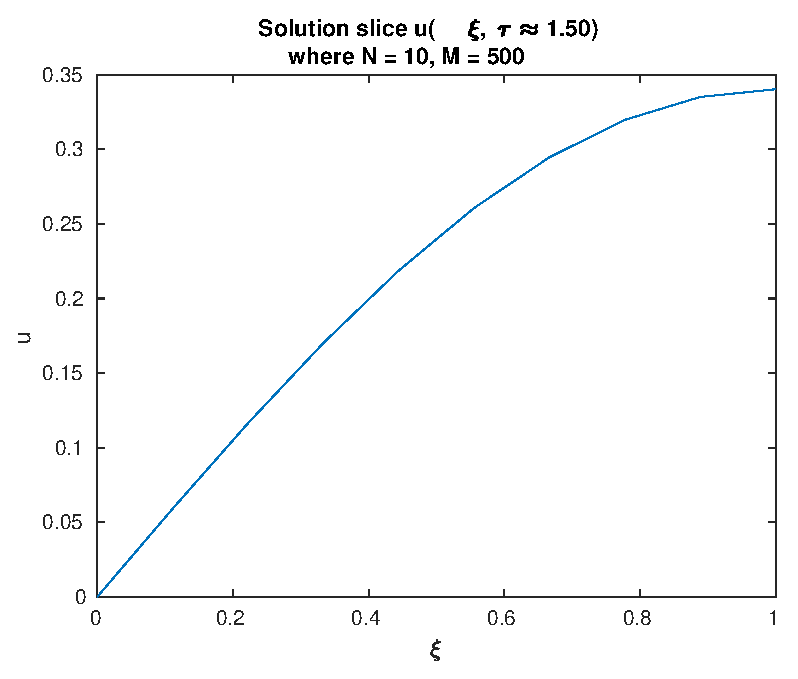
\includegraphics [width=4in]{lab3_05.eps}

\includegraphics [width=4in]{lab3_06.eps}

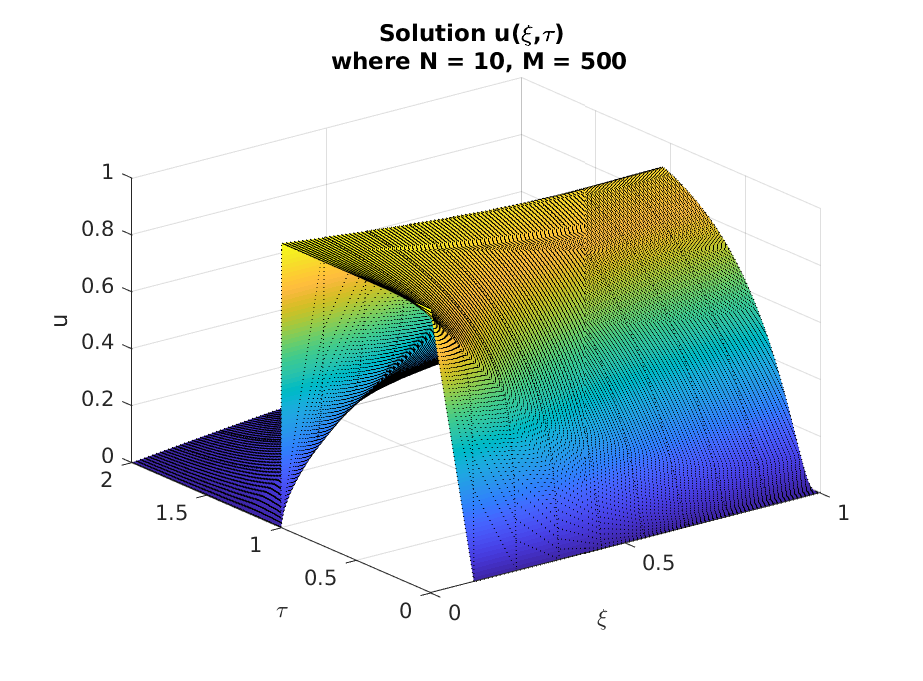
\includegraphics [width=4in]{lab3_07.eps}


\subsection*{Helper Functions}

\begin{par}
As always, helper functions are at the bottom.
\end{par} \vspace{1em}
\begin{verbatim}
function [A, b, xi, h] = mol_descretization(N)
% MOL_DESCRETIZATION returns parameters corresponding to the Method of
%                    Lines discretization of the nondimensional PDE
%                    described above.
%                    Returns
%                      xi - a vector of N xi points on [0, 1]
%                      b  - a function of tau generating a col vector of
%                           dim N-1 (as described above).
%                      A  - a matrix of dim N-1 x N-1 (as described above).
%                      h  - the grid spacing of xi.

% Generate spatial support.
xi = linspace(0, 1, N);  % NOTE: Includes xi_0 but not xi_N.
h = xi(2) - xi(1);

% Generate matrix A of dimensions N-1 x N-1.
dim = N-1;
diags = repmat((1/h^2) * [1 -2 1], dim, 1);   % Diagonals of A (mostly).
A = spdiags(diags, -1:1, dim, dim);           % Form A from diagonals.
A(end, end-1) = 2 * A(end, end-1);            % Update to account for BCs.

% Declare b as a function of tau.
b = @(tau) vertcat(1/h^2 * (tau <= 1), zeros(dim-1, 1));

end

function [xi, tau, U] = mol_ee_solve(N, M, tau_f)
% MOL_EE_SOLVE solves the nondimensional PDE described above with N spatial
%              grid points and M temporal grid points.
%              Uses Method of Lines and Explicit Euler.
%              Evolves until time tau_f.
%              Returns:
%                xi  - a vector of N xi points on [0, 1]
%                tau - a vector of M tau points on [0, tau_f]
%                U   - matrix were U(xi, tau) approximates u(xi, tau).
% See also lab3>mol_descretization.

% Get spatial MOL decretization parameters.
[A, b, xi, ~] = mol_descretization(N);

% Generate temporal support.
tau = linspace(0, tau_f, M);

% For convenience, store delta t.
dt = tau(2) - tau(1);

% For efficiency, we form dt*A + I just once instead of each iteration.
dtApI = dt*A + speye(size(A, 1));

% Allocate space for solution.
U = zeros(length(xi), length(tau));
% The above implicitly sets u^0 to zero (IC).
% We do have to manually account for U(1, :) since we removed it from the
% matrix system (corresponds to u^k_0 in write-up).
U(1, tau <= 1) = 1;

% Iterate over time steps.
% NOTE: k is 1-indexed here instead of 0-indexed like in the write-up.
for k = 1:M-1
    % NOTE: We are indexing rpws 2:end because we removed u_0.
    U(2:end, k+1) = dtApI * U(2:end, k) + dt * b(tau(k));
end
end

function [xi, tau, U] = mol_ode23_solve(N, tau_f, varargin)
% MOL_ODE23_SOLVE solves the nondimensional PDE described above with N
%                 spatial grid points.
%                 Uses Method of Lines and ode23[s].
%                 Evolves until time tau_f.
%                 After tau_f, any number of options may be passed in.
%                 Options:
%                   'stiff': uses a stiff solver.
%                   'jpat': passes JPattern to the solver (req. stiff).
%                   'jacob': passed jull jacobian to solver (req. stiff).
%                 Returns:
%                   xi  - a vector of N xi points on [0,1],
%                   tau - a vector of tau points on [0, tau_f].
%                   U   - matrix were U(j, k) approximates u(xi(j),tau(k)).
% See also lab3>mol_descretization.

use_stiff = false;
jpattern = false;
full_jacob = false;
for opt = varargin
    if strcmp(opt{:}, 'stiff')
        use_stiff = true;
    elseif strcmp(opt{:}, 'jpat')
        jpattern = true;
    elseif strcmp(opt{:}, 'jacob')
        full_jacob = true;
    end
end

% Get spatial MOL decretization parameters.
[A, b, xi, ~] = mol_descretization(N);

% Initialize solver options.
opts = odeset();

% Set solver to ode23 or ode23s based on use_stiff.
if use_stiff
    % If stiff, some other options may apply.
    solver = @ode23s;
    if full_jacob
        opts = odeset('Jacobian', A);
    end
    if jpattern
        opts = odeset('JPattern', (A ~= 0));
    end
else
    solver = @ode23;
end

    function dudt = mol_odefun(tau, u)
        % Computes du/dt for a given vector u and tau.
        dudt = A * u + b(tau);
    end

% Our odefun above is only valid for {u_1, ..., u_{N-1}).
dim = N-1;
u0 = zeros(dim, 1);  % First column of solution.
[tau, U] = solver(@mol_odefun, [0 tau_f], u0, opts);

% Since ode23[s] considers tau to be a column vector, and rows of U
% to be for fixed tau, we need to transpose both.
% In our write-up, cols of U are for fixed tau, and tau is a row vec.
tau = tau';
U = U';

% Prepend the row tau <= 1 to account for the eliminated u_0(tau).
U = vertcat(tau <= 1, U);
end
\end{verbatim}



\end{document}
    
